% TikZ figure for Darwin architecture
% Compile with: pdflatex architecture.tex

\documentclass[tikz,border=5pt]{standalone}
\usepackage{tikz}
\usetikzlibrary{shapes.geometric, arrows, positioning, fit, backgrounds}

\begin{document}

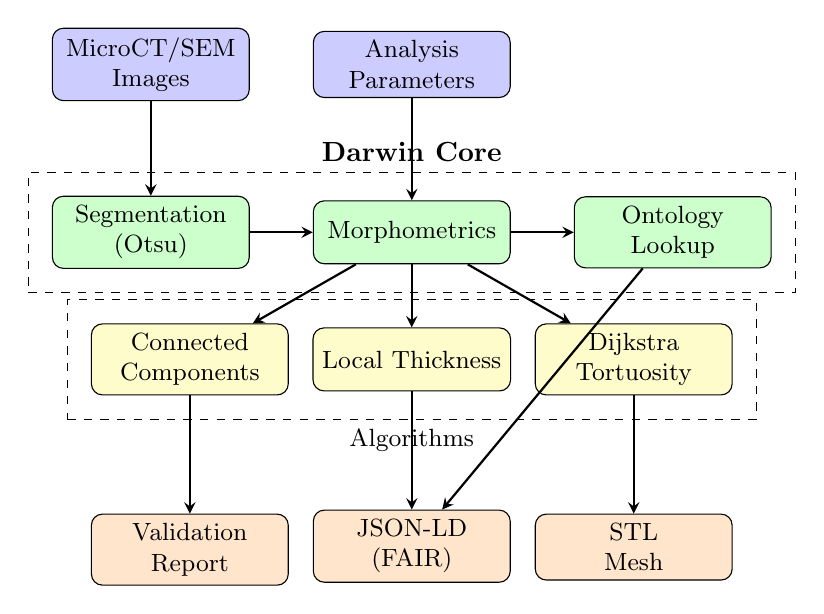
\begin{tikzpicture}[
    node distance=0.8cm,
    box/.style={rectangle, draw, rounded corners, minimum width=2.5cm, minimum height=0.8cm, align=center, font=\small},
    input/.style={box, fill=blue!20},
    process/.style={box, fill=green!20},
    output/.style={box, fill=orange!20},
    module/.style={rectangle, draw, dashed, inner sep=0.3cm},
    arrow/.style={->, thick, >=stealth}
]

% Input layer
\node[input] (microct) {MicroCT/SEM\\Images};
\node[input, right=of microct] (params) {Analysis\\Parameters};

% Processing modules
\node[process, below=1.2cm of microct] (segment) {Segmentation\\(Otsu)};
\node[process, right=of segment] (metrics) {Morphometrics};
\node[process, right=of metrics] (ontology) {Ontology\\Lookup};

% Algorithms
\node[box, below=0.8cm of metrics, fill=yellow!20] (lt) {Local Thickness};
\node[box, left=0.3cm of lt, fill=yellow!20] (cc) {Connected\\Components};
\node[box, right=0.3cm of lt, fill=yellow!20] (dijk) {Dijkstra\\Tortuosity};

% Outputs
\node[output, below=1.5cm of cc] (report) {Validation\\Report};
\node[output, below=1.5cm of lt] (jsonld) {JSON-LD\\(FAIR)};
\node[output, below=1.5cm of dijk] (stl) {STL\\Mesh};

% Arrows
\draw[arrow] (microct) -- (segment);
\draw[arrow] (params) -- (metrics);
\draw[arrow] (segment) -- (metrics);
\draw[arrow] (metrics) -- (ontology);

\draw[arrow] (metrics) -- (cc);
\draw[arrow] (metrics) -- (lt);
\draw[arrow] (metrics) -- (dijk);

\draw[arrow] (cc) -- (report);
\draw[arrow] (lt) -- (jsonld);
\draw[arrow] (dijk) -- (stl);
\draw[arrow] (ontology) -- (jsonld);

% Module boxes
\begin{scope}[on background layer]
\node[module, fit=(segment)(metrics)(ontology), label=above:{\textbf{Darwin Core}}] {};
\node[module, fit=(cc)(lt)(dijk), label=below:{\small Algorithms}] {};
\end{scope}

\end{tikzpicture}

\end{document}
